\chapter{Equations for the Motion of an Ideal-Fluid}
\section{Method of Analysis}
Two descriptions methods for fluid motion
\begin{enumerate}[label = (\arabic*)]
\item Lagrangian description\\
--tracing the motion of each fluid element (control-mass approach), i.e., $\mathbf{x} = \mathbf{x}(\boldsymbol{\xi},t)$ where $\boldsymbol{\xi}$ specifies the initial position of the fluid element, then
\begin{align*}
\mathbf{v}\equiv\left(\frac{\partial\mathbf{x}}{\partial t}\right)_{\boldsymbol{\xi}}&&\text{ and }&&\mathbf{a}\equiv\left(\frac{\partial^2\mathbf{x}}{\partial t^2}\right)_{\boldsymbol{\xi}}&&\text{etc.}
\end{align*}
\item Eulerian description \\
--recording fluid motion at each fixed location (field description, control-volume approach), i.e., $\mathbf{v} = \mathbf{v}(\mathbf{x},t)$ where $\mathbf{x}$ are fixed spatial coordinates.
\[
\therefore\mathbf{v}\neq \frac{\partial\mathbf{x}}{\partial t}.
\]
\end{enumerate}
Analysis can be classified as:
\begin{enumerate}[label = \protect\circled{\arabic*}]
\item Integral analysis-- Conservation laws being applied to a fixed region.
\item Differential analysis-- Conservation laws being applied, in a limiting case, to a point. This requires flow properties to be differentiable. 
\end{enumerate}

\section{Reynolds Transport Theorem (RTT)}
Laws of Mechanics are applied to a control-mass system (Lagrangian description). RTT converts the system analysis to an equivalent expression in control-volume approach (Eulerian description).
\begin{itemize}
\item Substantial derivative (time rate of change of properties following fluid motion)\\
Let $B(\mathbf{x},t)$ be a scalar (or vector) function, then 
%----------------------
\begin{minipage}{0.4\textwidth}
\begin{align*}
dB &= d\mathbf{x}\cdot\nabla B + \frac{\partial B}{\partial t}dt \\
\therefore
\frac{dB}{dt} &= \mathbf{v}\cdot B + \frac{\partial B}{\partial t}
\end{align*}
or 
\begin{equation}
\underbrace{\frac{DB}{Dt}}_
{
\begin{subarray}{c}
  \text{Lagrangian}\\
  \text{derivative}
\end{subarray}
}= \underbrace{\mathbf{v}\cdot\nabla B + \frac{\partial B}{\partial t}}_
{
\begin{subarray}{c}
  \text{equivalent}\\
  \text{Eulerian expression}
\end{subarray}
}
\label{eq: 2-1}
\end{equation}
\end{minipage} \hfill
\begin{minipage}{0.4\textwidth}
\begin{figure}[H]
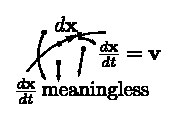
\includegraphics[scale=1.8]{figure/chapter2/2-1-1.eps}
%\caption{\label{fig:blue_rectangle} Rectangle}
\end{figure}
\end{minipage}
%----------------------
\item RTT \\
Let $\volume(t)$ be a closed region moving with the fluid (i.e. material volume) with boundary surface denoted by $S(t)$ and let $B(\mathbf{x},t)\footnotemark$ denote any \emph{intensive} property of the fluid field\footnotetext{could be scalar or vector function}, then

\begin{figure}[H]
\centering
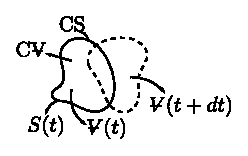
\includegraphics[scale=1.8]{figure/chapter2/2-1-2.eps}
%\caption{Scheme of blowing/suction flow}
%\label{Scheme of blowing/suction flow}
\end{figure}
\begin{subequations}
\label{eq: 2-2}
\begin{flalign}
\frac{D}{Dt}{\oiint \hspace{-23.5pt} \int}_{\volume(t)}\rho B d\volume
&\vc{=}{\footnotemark}{} {\oiint \hspace{-23.5pt} \int}_{\volume(t)}\frac{D\left(\rho B\right)}{Dt}d\volume + \rho B\frac{D\left(d\volume\right)}{Dt} \nonumber \\
&={\oiint \hspace{-23.5pt} \int}_{C\volume} \frac{D\left(\rho B\right)}{Dt}d\volume + \rho B\left(\nabla\cdot\mathbf{v}\right)d\volume \\
&= {\oiint \hspace{-23.5pt} \int}_{C\volume}\left[\frac{\partial\left(\rho B\right)}{\partial t} + \nabla\cdot\left(\rho B \mathbf{v}\right)\right]d\volume \\
&= {\oiint \hspace{-23.5pt} \int}_{C\volume}\frac{\partial\left(\rho B\right)}{\partial t}d\volume + \oiint_{CS}\mathbf{n}\cdot\left(\rho B\mathbf{v}\right)dS
\end{flalign}
\footnotetext{Recall $\displaystyle\nabla\cdot\mathbf{v} = \frac{1}{d\volume}\frac{D\left(d\volume\right)}{Dt}$, then $\displaystyle\frac{D\left(d\volume\right)}{Dt} = \left(\nabla\cdot\mathbf{v}\right)d\volume$}
\end{subequations}
\end{itemize}
\section{Differential Equations for an Ideal-Fluid Motion}
\begin{itemize}
\item Conservation of mass
\[
\frac{D}{Dt}{\oiint \hspace{-23.5pt} \int}_{\volume (t)}\rho d\volume = 0
\]
Apply RTT (set $B\equiv 1$) 
\begin{subequations}
\begin{align}[left = \empheqlbrace\,]
&{\oiint \hspace{-23.5pt} \int}_{C\volume}\frac{\partial\rho}{\partial t} d\volume + \underbrace{\oiint_{CS}\mathbf{n}\cdot\left(\rho \mathbf{v}\right)dS}_
{
\begin{subarray}{c}
  \text{net mass flow rate}\\
  \text{across CS (mass flux)}
\end{subarray}
}
= 0 \\
&{\oiint \hspace{-23.5pt} \int}_{C\volume}\left[\frac{\partial\rho}{\partial t} + \nabla\cdot\left(\rho\mathbf{v}\right)\right]d\volume = 0
\end{align}
\end{subequations}
Since C$\volume$ is \emph{arbitrary}
\begin{subequations}
\begin{align}
\Longrightarrow &\boxed{\frac{\partial\rho}{\partial t} + \nabla\cdot\left(\rho\mathbf{v}\right) = 0}\text{ everywhere} \\
\text{or }&\underbrace{\frac{\partial\rho}{\partial t}+\mathbf{v}\cdot\nabla\rho}_{\displaystyle\equiv\frac{D\rho}{Dt}} + \rho\nabla\cdot\mathbf{v} = 0\nonumber \\
\Longrightarrow & \frac{D\rho}{Dt} + \rho\nabla\cdot\mathbf{v} = 0
\end{align}
\end{subequations}
For an ideal fluid, $\rho =$ constant
\begin{align}
\Longrightarrow \frac{D\rho}{Dt} = 0&&\text{ or }&&\boxed{\nabla\cdot\mathbf{v} = 0}\text{ everywhere}
\end{align}
\item Conservation of Momentum
\begin{equation}
\frac{D}{Dt}{\oiint \hspace{-23.5pt} \int}_{\volume (t)}\rho\mathbf{v}d\volume = \sum\mathbf{F} = {\oiint \hspace{-23.5pt} \int}_{\volume (t)}\mathbf{f_b}d\volume + \oiint_{S(t)}\mathbf{f_s}dS
\tag{$\ast$} \label{eq: 2-*}
\end{equation}
where 
\begin{align*}
\mathbf{f_b}&\colon\text{body force/volume},\mathbf{f_b} = \rho\mathbf{g} \\
\mathbf{f_s}&\colon\text{surface force/area},\mathbf{f_s} = \mathbf{n}\cdot\boldsymbol{\tau}
\end{align*}
\[
\eqref{eq: 2-*}\Longrightarrow
\frac{D}{Dt}{\oiint \hspace{-23.5pt} \int}_{\volume (t)}\rho\mathbf{v}d\volume = {\oiint \hspace{-23.5pt} \int}_{\volume (t)}\rho\mathbf{g}d\volume + \oiint_{S(t)}\mathbf{n}\cdot\boldsymbol{\tau}dS
\]
Apply RTT (set $B=\mathbf{v}$)
\begin{subequations}
\begin{align}[left = \empheqlbrace\,]
&{\oiint \hspace{-23.5pt} \int}_{C\volume}\frac{\partial\left(\rho\mathbf{v}\right)}{\partial t} d\volume + \underbrace{\oiint_{CS}\mathbf{n}\cdot\left(\rho \mathbf{v}\mathbf{v}\right)dS}_
{
\begin{subarray}{c}
  \text{net momentum flux}\\
  \text{across CS}
\end{subarray}
}\nonumber \\
&= {\oiint \hspace{-23.5pt} \int}_{C\volume }\rho\mathbf{g}d\volume + \oiint_{CS}\mathbf{n}\cdot\boldsymbol{\tau}dS \\
&{\oiint \hspace{-23.5pt} \int}_{C\volume}\frac{\partial\left(\rho\mathbf{v}\right)}{\partial t} d\volume + \oiint_{C\volume}\nabla\cdot\left(\rho \mathbf{v}\mathbf{v}\right)d\volume \nonumber\\ 
&= {\oiint \hspace{-23.5pt} \int}_{C\volume }\rho\mathbf{g}d\volume + {\oiint \hspace{-23.5pt} \int}_{C\volume }\nabla\cdot\boldsymbol{\tau}d\volume
\end{align}
\end{subequations}
Since C$\volume$ is \emph{arbitrary}
\begin{subequations}
\begin{align}
\Longrightarrow &\frac{\partial\left(\rho\mathbf{v}\right)}{\partial t} + \nabla\cdot\left(\rho \mathbf{v}\mathbf{v}\right) = \rho\mathbf{g} + \nabla\cdot\boldsymbol{\tau} \\
&\text{Use }\nabla\cdot\left(\rho\mathbf{v}\mathbf{v}\right) = \left[\nabla\cdot\left(\rho\mathbf{v}\right)\right]\mathbf{v} + \rho\mathbf{v}\cdot\left(\nabla\mathbf{v}\right) \nonumber\\
&\text{and apply continuity equation}\nonumber\\
\Longrightarrow &\underbrace{\rho\frac{\partial\mathbf{v}}{\partial t} + \rho \mathbf{v}\cdot\nabla\mathbf{v}}_{\displaystyle =\rho\frac{D\mathbf{v}}{Dt}} = \rho\mathbf{g} + \nabla\cdot\boldsymbol{\tau} \label{eq: 2-7b}
\end{align}
\end{subequations}
For an ideal fluid, $\mu = 0$,
\[
\boldsymbol{\tau} = -p\mathbf{I}\text{ only}
\]
hence \eqref{eq: 2-7b} reduce to
\begin{equation}
\boxed{\rho\frac{D\mathbf{v}}{Dt} = \rho \mathbf{g} - \nabla p}\text{ (Euler equation)}
\label{eq: 2-8}
\end{equation}
\item Conservation of Energy (1\textsuperscript{st} law of thermodynamics)
\begin{multline*}
\frac{D}{Dt}{\oiint \hspace{-23.5pt} \int}_{\volume (t)}\rho\left(e + \frac{v^2}{2}\right)d\volume = \sum\mathbf{F}\cdot\mathbf{v} \\
= {\oiint \hspace{-23.5pt} \int}_{\volume (t)}\mathbf{f_b}\cdot\mathbf{v}d\volume + \oiint_{S(t)}\mathbf{f_s}\cdot\mathbf{v}dS - \oiint_{S(t)}\mathbf{n}\cdot\mathbf{\dot{q}}dS \\
= {\oiint \hspace{-23.5pt} \int}_{\volume (t)}\rho\mathbf{g}\cdot\mathbf{v} d\volume + \oiint_{S(t)}\left(\mathbf{n}\cdot\boldsymbol{\tau}\right)\cdot\mathbf{v}dS + \oiint_{S(t)}\mathbf{n}\cdot\left(k\nabla T\right)dS
\end{multline*}
where 
\begin{align*}
e&\colon\text{internal energy/mass} \\
\frac{v^2}{2}&\colon\text{macro kinetic energy/mass}
\end{align*}
Apply RTT (set $B=e+v^2/2$)
\begin{subequations}
\begin{align}[left = \empheqlbrace\,]
&{\oiint \hspace{-23.5pt} \int}_{C\volume}\frac{\partial}{\partial t}\left[\rho\left(e+\frac{v^2}{2}\right)\right] d\volume \nonumber \\ 
&+ \underbrace{\oiint_{CS}\mathbf{n}\cdot\left[\rho\left(e+\frac{v^2}{2}\right)\right]dS}_
{
\begin{subarray}{c}
  \text{net energy flux}\\
  \text{across CS}
\end{subarray}
}\nonumber \\
&= {\oiint \hspace{-23.5pt} \int}_{C\volume }\rho\mathbf{g}\cdot\mathbf{v} d\volume + \oiint_{CS}\left(\mathbf{n}\cdot\boldsymbol{\tau}\right)\cdot\mathbf{v}dS\nonumber \\
& + \oiint_{CS}\mathbf{n}\cdot\left(k\nabla T\right)dS\\
&{\oiint \hspace{-23.5pt} \int}_{C\volume}\frac{\partial}{\partial t}\left[\rho\left(e+\frac{v^2}{2}\right)\right] d\volume \nonumber \\ 
&+ {\oiint \hspace{-23.5pt} \int}_{C\volume}\nabla\cdot\left[\rho\left(e+\frac{v^2}{2}\right)\right]d\volume\nonumber \\
&= {\oiint \hspace{-23.5pt} \int}_{C\volume }\rho\mathbf{g}\cdot\mathbf{v} d\volume + {\oiint \hspace{-23.5pt} \int}_{C\volume}\nabla\cdot\left(\boldsymbol{\tau}\cdot\mathbf{v}\right)d\volume\nonumber \\
& + {\oiint \hspace{-23.5pt} \int}_{C\volume}\nabla\cdot\left(k\nabla T\right)d\volume
\end{align}
\end{subequations}
Since C$\volume$ is \emph{arbitrary}
\begin{subequations}
\begin{align}
\Longrightarrow &\frac{\partial}{\partial t}\left[\rho\left(e+\frac{v^2}{2}\right)\right] + \nabla\cdot\left[\rho\left(e+\frac{v^2}{2}\right)\right]\nonumber\\ 
&= \rho\mathbf{g}\cdot\mathbf{v} + \nabla\cdot\left(\boldsymbol{\tau}\cdot\mathbf{v}\right)  + \nabla\cdot\left(k\nabla T\right)\\
&\text{Use continuity/momentum equation}\nonumber\\
\Longrightarrow &\rho \frac{D}{Dt}\left[\rho\left(e+\frac{v^2}{2}\right)\right]\nonumber\\ 
&= \rho\mathbf{g}\cdot\mathbf{v} + \nabla\cdot\left(\boldsymbol{\tau}\cdot\mathbf{v}\right)  + \nabla\cdot\left(k\nabla  T\right)\label{eq: 2-10b}
\end{align}
\end{subequations}
For an ideal fluid, 
$
\left\{
\begin{aligned}
\rho = \text{ constant}&\Longrightarrow \nabla\cdot\mathbf{v} = 0 \\
\mu = 0&\Longrightarrow\boldsymbol{\tau} = -p\mathbf{I}
\end{aligned}
\right.
$
hence \eqref{eq: 2-10b} reduce to
\begin{equation}
\rho \frac{D}{Dt}\left[\rho\left(e+\frac{v^2}{2}\right)\right] = \rho\mathbf{g}\cdot\mathbf{v}-\nabla\cdot\left(p\mathbf{v}\right) + \nabla\left(k\nabla T\right)\tag{$\ast$}\label{eq: 2-1-*}
\end{equation}
From momentum equation \eqref{eq: 2-8} perform
\begin{equation}
\mathbf{v}\cdot\left\{\rho\frac{D\mathbf{v}}{Dt} = \rho \mathbf{g} - \nabla p\right\}\tag{$\ast\ast$}\label{eq: 2-1-**}
\end{equation}
notice that
\begin{align*}
\mathbf{v}\cdot\left[\mathbf{v}\cdot\nabla\mathbf{v}\right]
&= \mathbf{v}\cdot\left[\nabla\left(\frac{v^2}{2}\right) - \mathbf{v}\times\underbrace{\left(\nabla\times\mathbf{v}\right)}_{=\boldsymbol{\xi}}\right] \\
&= \mathbf{v}\cdot\nabla\left(\frac{v^2}{2}\right)  - \underbrace{\mathbf{v}\cdot\left(\mathbf{v}\times\boldsymbol{\xi}\right)}_{=0}
\end{align*}
hence \eqref{eq: 2-1-**}
\begin{equation}
\Longrightarrow\rho\frac{ D}{Dt}\left(\frac{v^2}{2}\right) = \rho \mathbf{g}\cdot\mathbf{v} - \mathbf{v}\cdot\nabla p
\label{eq: 2-1-11}
\end{equation}
Subtract \eqref{eq: 2-1-11} from \eqref{eq: 2-1-*}
 \begin{equation}
\Longrightarrow\rho\frac{ De}{Dt} =  - \mathbf{v}\cdot\nabla p + \nabla\cdot\left(k\nabla T\right)
\label{eq: 2-1-12}
\end{equation}
For ideal fluid, $\nabla\cdot\mathbf{v} = 0$ and non-conducting, $k=0$,
\[
\Longrightarrow\boxed{\frac{De}{Dt} = 0}
\]
Thus, don't need energy equation when dealing with ideal flows.
\end{itemize}
\section{Boundary Condition for an Ideal-Fluid Motion}
\begin{itemize}
\item At solid-fluid boundary-- No penetration condition
%----------------------
\begin{minipage}{0.4\textwidth}
\begin{equation}
\boxed{\mathbf{v}\cdot\mathbf{n} = \mathbf{v_s}\cdot\mathbf{n}}
\label{eq: 2-13}
\end{equation}
\end{minipage} \hfill
\begin{minipage}{0.4\textwidth}
\begin{figure}[H]
\centering
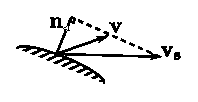
\includegraphics[scale=1.8]{figure/chapter2/2-1-3.eps}
%\caption{\label{fig:blue_rectangle} Rectangle}
\end{figure}
\end{minipage}\\
%----------------------
If body is fixed, $\mathbf{v_s} = \mathbf{0}$
\begin{equation}
\eqref{eq: 2-13}\Longrightarrow\boxed{\mathbf{v}\cdot\mathbf{n} = 0}
\label{eq: 2-14}
\end{equation}
i.e., fluid can only slide on the solid body surface.
\item At fluid-fluid boundary\\
Assume immiscible situation
\begin{enumerate}[label = (\alph*)]
\item Kinematic conditions\\
Let $F(\mathbf{x},t)=0$ represents the instantaneous  position of the interface, then\\
%----------------------
\begin{minipage}{0.2\textwidth}
\begin{align}
&\boxed{\mathbf{v_A}\cdot\mathbf{n} = \mathbf{v_B}\cdot\mathbf{n}}\label{eq: 2-15} \\
&\text{ or }\left(\mathbf{v_A}-\mathbf{v_B}\right)\cdot\underbrace{\nabla F}_{\parallel\mathbf{n}} = 0\nonumber
\end{align}
\end{minipage} \hfill
\begin{minipage}{0.4\textwidth}
\begin{figure}[H]
\centering
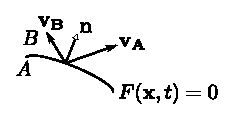
\includegraphics[scale=1.8]{figure/chapter2/2-1-4.eps}
%\caption{\label{fig:blue_rectangle} Rectangle}
\end{figure}
\end{minipage}\\
%----------------------
but the tangential components may be different across the interface $\Longrightarrow$ surface of tangential discontinuity.\\
e.g. 
\begin{figure}[H]
\centering
\subfigure[Ideal-Fluid flow]
{
%\label{3-7-Plot of frequency response in amplitude}
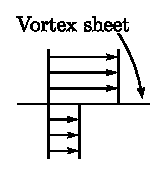
\includegraphics[scale=1.5]{figure/chapter2/2-1-5-a.eps}
}
\centering
\subfigure[Real flow]
{
%\label{3-7-Plot of frequency response in phase}
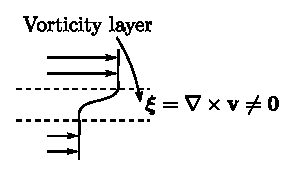
\includegraphics[scale=1.5]{figure/chapter2/2-1-5-b.eps}
}
%\caption{Plot of frequency response}
\end{figure}
\item Dynamic condition\\
%----------------------
\begin{minipage}{0.4\textwidth}
\begin{figure}[H]
\centering
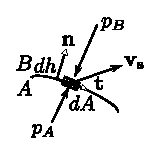
\includegraphics[scale=1.8]{figure/chapter2/2-1-6.eps}
%\caption{\label{fig:blue_rectangle} Rectangle}
\end{figure}
\end{minipage} \hfill
\begin{minipage}{0.4\textwidth}
Take a small element moving with the interface $dhdA$ over a segment of the interface, the force balance equation in the $\mathbf{n}-$direction
\end{minipage}\\
%----------------------
\[
f_{bn}dAdh + \left(p_A-p_B\right)dA - \underbrace{\sum a_{\text{rel},n}\left(\rho dA dh\right)}_{\text{Apparent force terms}} = 0
\]
\begin{equation}
\text{As } dh\to 0\Longrightarrow\boxed{p_A=p_B}
\label{eq: 2-16}
\end{equation}
\end{enumerate}
\end{itemize}